\begin{figure}[!htpb] 
\begin{center}
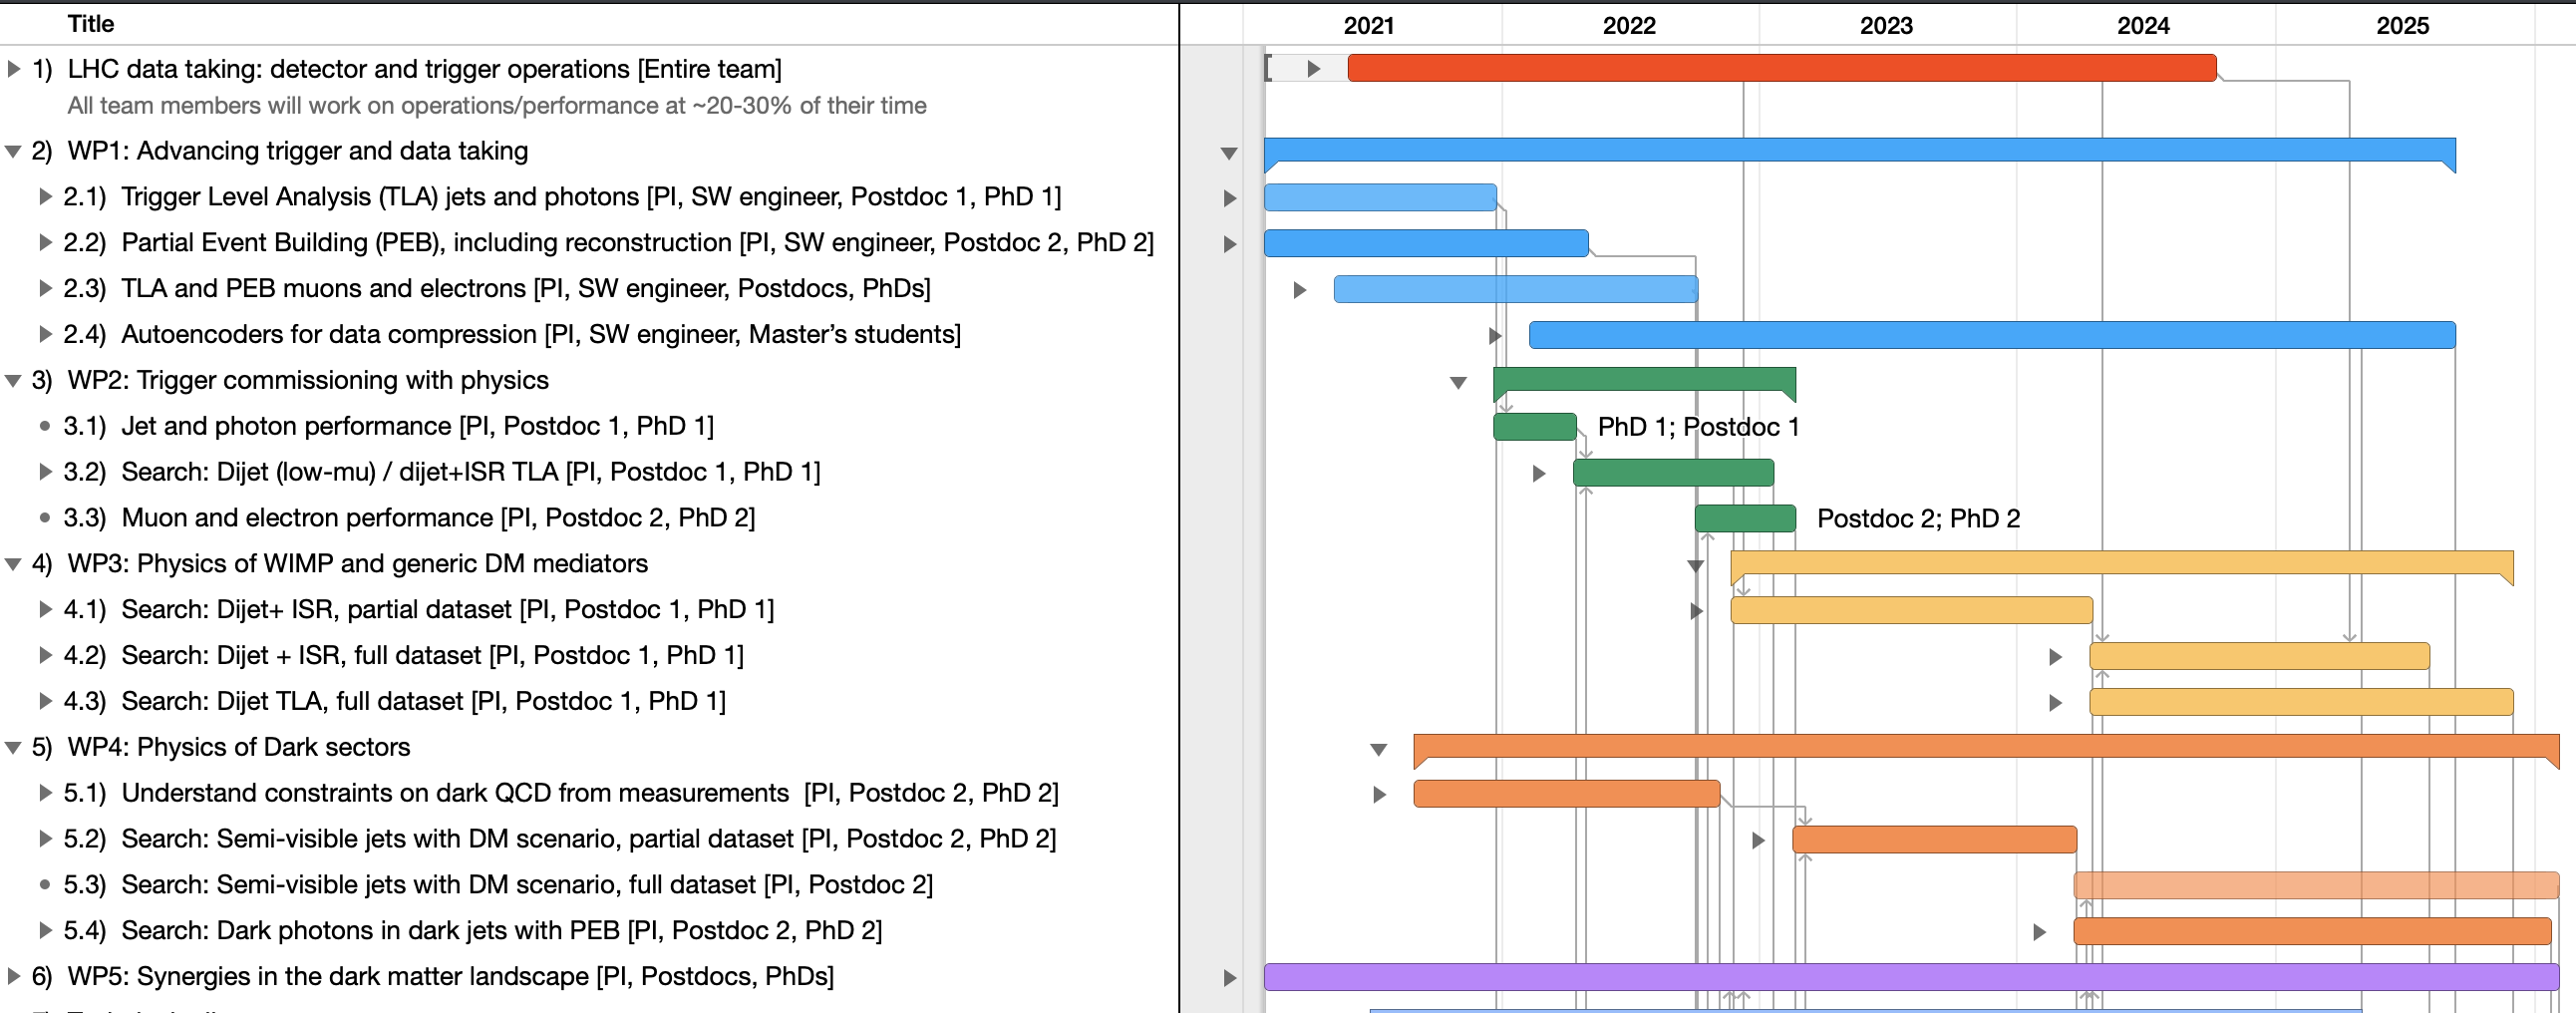
\includegraphics[width=\textwidth]{figs_B2/gantt}
\caption{\color{black}\label{fig:gantt} \small Sketch of project planning and division of work across team members.} 
\vskip2pt
\end{center}
\end{figure}
%\vskip5pt

The research team of \textsc{Realdark} that I will lead as a PI is composed by two postdoctoral researchers, two PhD students and one software engineer.
%Shift this to Resources
The postdoctoral researchers (PD1 and PD2) will be employed for the entirety of the project. 
The PhD students (PhD1 and PhD2) will work within \textsc{Realdark} for their 4-year thesis period. 
Each of the postdocs will work with one of the PhD students on the two physics objectives of WP3 and WP4 respectively, and related technical and commissioning tasks in WP1 and WP2. 
As PI, I will oversee all tasks in the project with day-to-day supervision and regular meetings, and have a hands-on involvement in more complex tasks as specified below. 
%allowing an effective sharing of supervision tasks. 
The software engineer will have a two-year contract at the beginning of the project to ensure the feasibility of the more software-intensive tasks in WP1. 
%end of shift to resources
Fig.~\ref{fig:gantt} provides a project planning schedule, including the breakdown of the work between the team members and intermediate milestones and deliverables marked with \textbf{[N]}. 
It has been prepared using the OmniPlan software~\ref{ToBeCited},%Omniplan 
taking into account the interdependencies between the WPs and 
scheduling the work allocation in a way that ensures the feasibility of this ambitious project without overcommitting the team members. 

\subsection{WP1: Real-time analysis and data compression in ATLAS}

%The software implementation of TLA and TLA+PEB techniques and the calibration of physics objects recorded using these techniques represents a significant portion of the work in WP1. 
\textbf{TLA software implementation and calibration of trigger objects} As a preliminary input to this proposal, I have started working on a new Run-3 multithreaded HLT software algorithm that selects and writes out partially-built physics objects in the TLA stream. 
This algorithm will be more flexible than its Run-2 counterpart, and can handle any physics objects. 
By the start of this proposal, we will have preliminary results of the use of this algorithm on TLA jets. 
In 2021, PI, PD1, PhD1 and the software engineer
will work on the readiness of the core software for photons and jets, on commissioning with cosmic data, and on their subsequent calibration \textbf{[1]}
The experience gained with photons will be used by P1 and PhD1 to implement and commission TLA electrons as well \textbf{[2]}, while PD2 and PhD2 will focus on TLA muons \textbf{[3]}. 
Initially, the TLA stream will contain both jets and photons to enable analyses in WP3 in a simple manner. 
As part of this work, we will contribute to the design and implementation of seed trigger chains and data streams that selectively record one or more TLA objects simultaneously, optimizing according to the use cases in WP3 and WP4. 
The finalized TLA software streams will be ready in Q3 2022, allowing sufficient time for validation with data prior to the LHC production period. \\
\textbf{PEB software implementation and reconstruction} Prior to the implementation of TLA muons (Q1-Q2 2021), PD2 and PhD2 will deploy the core software to write out user-defined regions of the detector together with TLA objects, 
%based on the Run-2 example for muons~\cite{ToBeCited}  and 
taking into account the optimization between CPU and storage costs mentioned in Sec.~\ref{subsub:TriggerRecoSoftware}. 
%strike a balance between the use of computing-expensive HLT algorithms to be able to drop raw detector data, and delaying running those algorithms until later at the cost of a larger event size. 
%The Cost Monitoring framework and test events storing different levels of detector information, informed by the calibration and reconstruction work as well as by the sensitivity studies, will be evaluated for this optimization. 
Subsequently, they will test the TLA+PEB implementation on early data and work together with the software engineer on the implementation of dedicated reconstruction algorithms for partial detector input, taking advantage of the experience gained with TLA electrons and muons~\textbf{[4]}. 
At the end of this work, expected for Q3 2022, we will publish a technical paper describing the combined TLA and PEB implementation within the ATLAS trigger (Q4 2022) \textbf{[5]}. \\
\textbf{Identification and calibration of TLA jets, photons, electrons and muons} Throughout 2021 and 2022, PhDs and postdocs will contribute to the algorithms for the identification and calibration of the HLT physics objects that they have implemented in TLA and PEB. 
In this proposal, we will focus on new HLT pile-up suppression techniques using calorimeter information against techniques using tracking information. 
The performance of this calibration will be studied in WP2 and documented in the technical papers in \textbf{[5]} and \textbf{[10]}.\\
Together with the performance studies, this work will be part of the students' ATLAS authorship qualification task.
\textbf{Data compression with autoencoders} Throughout the course of this proposal, the software engineer and I will supervise Master's students that study the performance, implementation and characteristics of autoencoder networks used to compress ATLAS data. 
The outcome of this work will be a test implementation in system that emulates a HLT computing node, preparing the ground for an implementation in the HL-LHC trigger and computing system~\textbf{[7]}. 
This work will be documented in technical publications, detailing preliminary and final work \textbf{[6,8]}.

\subsection{WP2: Commissioning the upgraded ATLAS trigger with physics}

\textbf{HLT object performance} Over the course of the early LHC data taking (2021-2022), 
PD1 and PhD1 will determine the performance of HLT jets and photons with early data, while PD2 and PhD2 will focus on the performance of HLT and PEB electrons and muons. \\
\textbf{Searches and measurements of the dijet mass spectrum} After the trigger jet and photon performance is well understood, PD1 and PhD1 and I will measure the dijet mass spectrum using a limited amount of data. 
We will select inclusive dijet events, and events where dijets produced in association with a photon, first using offline jets and TLA jets, and then using TLA+PEB jets, for comparison with simulation and Run-2 data. 
This will lead to a prototype of the dijet and dijet+ISR TLA searches within the RECAST framework~\textbf{[9]}.   
PD2 and PhD2 will repeat this exercise with electrons and muons in a measurement of the $Z$ and $J/\psi$ peaks, 
to be included with the jet and photon performance work in a dedicated technical publication~\textbf{[10]}. 
If the LHC provides a dataset that surpasses the Run-2 sensitivity for either dijet and dijet+ISR searches, 
PD1, PhD1 and I will work with ATLAS collaborators towards publication of the result of these searches in Q2 2023~\textbf{[11]}.

\subsection{WP3: Dark matter mediator searches}

WIMP mediator searches and the interpretation of their results will be the main physics focus of PD1 and PhD1.
\textbf{Dijet+ISR TLA search} This search relies on calibrations and data analysis code developed and tested in WP1 and WP2.
%PD1 and PhD1 will perform the sensitivity and literature studies to deploy trigger chains seeding these TLAs prior to 2022, 
PD1 and PhD1 will refine the WP1 jet calibration for a high-statistics search (e.g. for pile-up suppression suppression techniques for the low-$p_{\mathrm{T}}$ resonance jets) and repeat the performance studies from WP2 with a larger dataset. 
PD1 and PhD1 will take advantage of WP2 RECAST implementation of the dijet+ISR mass spectrum to estimate backgrounds and produce inputs to run the statistical analysis.
PD1 and PhD1 will collaborate with colleagues from OSU, Oregon and other ATLAS institutes for two publications, one using the first part of the dataset where the Run-2 sensitivity is surpassed~\textbf{[12]} in 2024, and one using the full Run-2 dataset~\textbf{[13]} in Q2 2025.\\ 
\textbf{Dijet TLA search} PD1 and I will remain involved in the full ATLAS Run-3 TLA with an advisory role. 
We will provide the WP2 RECAST implementation, and combine Run-2 and Run-3 results for a legacy TLA publication covering both LHC runs in Q3 2025 \textbf{[14]}. 
Dijet searches are sensitive to a variety of new physics signals (see Sec.~\ref{sub:stateOfTheArtTheory}): code and results from WP3 searches will be input to WP5 for broad dissemination. 

\subsection{WP4: Dark QCD searches}

Dark QCD searches and the interpretation of their results will be the main physics focus of PD2 and PhD2. 
Both searches in WP4 will require preliminary work and collaborations to decide on the optimal parameter space to target, described in WP5 below. 
This will be done within the first and second year of this proposal and culminate in a public document (ATLAS PUB note) on the reinterpretation of measurements and existing searches for a variety of dark QCD benchmark models in Q3 2022. 
This will inform the configuration for the TLA+PEB stream to be implemented upon the LHC restart in Q1-Q2 2023, 
together with the preliminary studies on the suppression of QCD background to implement at the HLT. \\
\textbf{Semi-visible jet search} This search will be the first to be tackled.
% as it relies on studies and analysis code in WP1-3 given the relative similarity of the two signatures. 
PD2 and PhD2 will bring their expertise to search for low-mass particles decaying into semi-visible jets in TLA+PEB, and work with colleagues from the University of Witswatersrand who will focus on the high-mass region with traditional techniques. 
This continues an existing collaboration started within my StG, which we expect to be supported by the ERC "Implementing Agreements" program during 2020.
We will publish this search with an intermediate dataset in Q2 2024~\textbf{15}, and continue our involvement in the full-dataset search with an advisory role. \\
\textbf{Composite jet search} This shares many of the common PEB+TLA performance tools with the semi-visible jet search and proceeds in parallel during 2023. 
The bulk of the work will be done during 2024, first adapting WP1 and WP2 code and techniques for leptons within jets and then running the analysis chain, leading to a publication in Q4 2025~\textbf{16}. 
Throughout this period we will also work to make the TLA+PEB stream and the analysis tools available within ATLAS for other dark sector searches. 

\subsection{WP5: Interpretation, dissemination and synergies}

The work in WP5 is spread over all the timeline of this project and its hands-on components will involve the PI, the postdocs and the PhDs.
A \textbf{two-weeks workshop} with other non-LHC communities, involving experts and authors of the theory benchmarks for searches in this proposal who agreed to participate~\cite{ToBeCited} %Felix & co
will be organized in Q3 2021 within the iDMEu initiative. 
The workshop will be hosted at Lund for the first week and at CERN for the second week (with videoconference available in both), to discuss the state-of-the-art of dark QCD theory and experiment and understand current constraints including dark meson searches, non-collider and astrophysical constraints. \\
Together with each technical and physics publication we will share our results on HEPData and on plots that summarize searches from different techniques and experiments constraining the same model. Within iDMEu, we will also extend the benchmarks for these plots to dark QCD models, with a first iteration expected after the Lund/CERN workshop. \\
We will also make common-interest software in WP1 (e.g. compression, non-standard object reconstruction) and WP2-4 (RECAST analyses in REANA) available in the ESCAPE Software Catalogue as part of the DM Virtual Environment, and on the HSF webpages. 
This will include documentation and working examples for enhancing the usability and impact of the shared software. \\
Finally, I will write a review of the state of the art of LHC searches at colliders at the end of this project~\textbf{[17]}. 

%\textbf{Defining search targets} 
%Through workshops and discussions with the theory community, PD2 
%\textbf{Performance studies} During Q, the performance studies in WP2 will be extended to muons and electrons in busier hadronic environments, with a focus on the identification of variables and analysis techniques that can be used to minimize the impact of pile-up and reduce SM backgrounds already at the trigger level. 


%%%%%%BEGIN TO COMPILE UP TO HERE 
\clearpage
\begingroup
    \setboolean{inbibliography}{true}
\bibliographystyle{LHCb}
    \linespread{0.9}\selectfont
\bibliography{researchrefs}
\endgroup
%{\bf Note:} The PI is an author of Refs.~\cite{LHCb-PUB-2014-027,Bourgeois:2018nvk} and all the LHCb collaboration papers, with particular contributions to  Refs.~\cite{Aaij:2014jba,CERN-LHCC-2014-016,Aaij:2013mga,Aaij:2014ywt,LHCb-PUB-2014-040,Aaij:2016kjh,Aaij:2017lff}.
%The PI is acknowledged in Ref.~\cite{Jung:2014jfa}.
\end{document}  
%%%%%%END TO COMPILE UP TO HERE 

These studies will also give sufficient handles to understand the variability of QCD jets to evaluate search sensitivity and systematic uncertainties.
They will also provide input to a parallel effort funded by my VR Project Grant focused on anomaly detection techniques.  




 with lower thresholds with respect to offline searches, with sufficient raw detector information in the region behind the jets. 
 


Designing an HLT pre-selection that 
Rejecting sufficient QCD background with an HLT pre-selection will 

Preliminary work to understand the performance 





PD2 and PhD2 will focus on dark sector searches, using data recorded with the TLA+PEB technique for dark QCD searches. 

The work in WP1 and WP2 on the reconstruction, calibration and performance of regional detector data will be the stepping stone for the searches for semi-visible jets and composite jets. 
In WP4, we will \textbf{extend the study of isolated object performance to busier hadronic environments}, with a focus on the identification of variables and analysis techniques that can be used to minimize the impact of pile-up and reduce SM backgrounds already at the trigger level \textbf{[15]}. 
Rejecting sufficient QCD background with a pre-selection will allow recording higher rate of TLA+PEB events with lower thresholds with respect to offline searches, with sufficient raw detector information in the region behind the jets. 
These studies will also give sufficient handles to understand the variability of QCD jets to evaluate search sensitivity and systematic uncertainties.
They will also provide input to a parallel effort funded by my VR Project Grant focused on anomaly detection techniques.  
The \textbf{search for semi-visible jets} will be performed first~\textbf{[16]}, after we have reached sufficient understanding of the hadronic jet content. 
Subsequently, we will augment the standard reconstruction techniques to correctly identify anomalous content (e.g. leptons in jets) needed for the \textbf{composite jet search}~\textbf{[17]}.

An additional advantage of the PEB+TLA data stream selected for these searches is that it enables searches for a wide variety of non-standard jet topologies (e.g. photon-jets~\cite{PhotonJets}, jets containing long-lived particles~\cite{PhotonJets}) at a later date. 
This will have an impact especially after the end of this proposal when the long LHC shutdown is foreseen before HL-LHC and data already taken will be analyzed in further detail. 


\subsection{WP5: Dissemination and synergies}
\textbf{Organization of workshops} 
\textbf{Dissemination of results and summary plots} 
\textbf{Sharing of tools} 


%%%%%%BEGIN TO COMPILE UP TO HERE 
\clearpage
\begingroup
    \setboolean{inbibliography}{true}
\bibliographystyle{LHCb}
    \linespread{0.9}\selectfont
\bibliography{researchrefs}
\endgroup
%{\bf Note:} The PI is an author of Refs.~\cite{LHCb-PUB-2014-027,Bourgeois:2018nvk} and all the LHCb collaboration papers, with particular contributions to  Refs.~\cite{Aaij:2014jba,CERN-LHCC-2014-016,Aaij:2013mga,Aaij:2014ywt,LHCb-PUB-2014-040,Aaij:2016kjh,Aaij:2017lff}.
%The PI is acknowledged in Ref.~\cite{Jung:2014jfa}.
\end{document}  
%%%%%%END TO COMPILE UP TO HERE 


%In particular, the performance of trigger-level photons obtained in Run-2~\cite{ToBeCited} %EGamma paper
%and preliminary studies performed by a Lund Bachelor’s student~\cite{ToBeCited}%LeoBachelorThesis
%already give sufficient confidence on the feasibility of a dijet+ISR search, where the resonance is built from the jets and the photon is used as a tag. 
%The main challenge for this search lies in distinguishing low-$p_{\rm{T}}$ hard-scatter jets from pile-up jets, and efficiently subtracting pile-up contributions. 

%Project planning


%While TLA events are already reconstructed at the HLT and only need to be calibrated (see next section), in the case of the TLA+PEB stream we will need to adapt the offline software reconstruction algorithms to be able to cope with receiving partial detector data as input. 

%%%%%%%%%%%%


\subsubsection{Optimization of trigger resources}

Given that a large part of the searches in this proposal occurs at the HLT, a resource constrained environment, an important part of the planning prior to data taking is to optimize the CPU and storage resources needed for each of the searches. After this optimization, we can deploy the dedicated trigger chains to select events that will be analyzed using the TLA or the TLA+PEB techniques. 

In the case of TLA, where reconstruction and a near-final calibration of objects need to be performed in the HLT farm, we will estimate the CPU costs of various options using the ATLAS Cost Monitoring framework~\cite{CostMonitoringTim}, prior to data taking in 2021.  
Preliminary estimates are already available for the dijet+ISR photon analysis based on Run-2 software, indicating that this is expected, but further optimizations will be possible taking advantage of the rewrite of the trigger software and of the improved tracking and accounting for the early LHC running conditions (e.g. low luminosity runs) that will be known over the course of 2020. Using those new estimates, we will adjust the thresholds of the trigger chains and the level of precision of the algorithms used to maximize the sensitivity of the TLA dijet and dijet+ISR searches, based on the studies in Sec.\ref{sub:SensitivityStudies}. 
 

%%%%%


\subsubsection{Data preparation}


In this proposal “data preparation” indicates the series of methods and procedures that are needed to transform the raw data into final distributions. For non-standard analyses such as TLA and TLA+PEB, these procedures differ with respect to traditional analysis, as more of this process needs to be customized and controlled by the analysis team. 

In brief, the steps taken in this process are:

\begin{itemize}

\item Data are recorded by ATLAS using the trigger chains designed in Sec.~\ref{sec:OptimizationOfResources}. This is when real-time reconstruction of the data happens in the HLT computing farm, and its outputs are directly sent to the TLA stream;
\item A small fraction of data are reconstructed and analyzed right away as data taking occurs for monitoring purposes (both centrally and by the analysis team, using the toolkit in Sec.~\ref{sec:Performance})
\item Raw data, TLA and TLA+PEB data in \textit{bytestream} format are stored on tape at the CERN data center (Tier-0). 
Raw detector data is reconstructed shortly after having been taken, requiring most of the Tier-0 computing resources. 
TLA data requires fewer computing resources at this stage, as it already contains reconstructed objects. 
TLA+PEB data is not reconstructed immediately, but rather transferred to local resources where specialized reconstruction algorithms can be ran, or processed when the LHC is not running~\footnote{This is a procedure I was instrumental in defining and using in Run-1 and Run-2, called “delayed stream” in ATLAS or “data parking” in CMS}. 
\item Reconstructed data are processed from \textit{bytestream} format to a user-readable data format, called \textit{AOD}.  

\end{itemize}

From this point on, AOD data are sent to computing centers worldwide where user analysis occurs. User analysis includes:

\begin{itemize}
\item Derivation of the calibration constants and of their uncertainties. This step is generally done centrally by the experiment’s “Combined Performance groups”. We will participate actively to this work that is useful for the entirety of ATLAS, and customize central recommendations wherever needed for the analyses in WP3 and WP4. 
\item Application of updated calibration constants to the data used for analysis and to the simulation of signal and backgrounds.  
\item Production of final distributions of the observables needed for the monitoring of calibration performance and for further data analysis. This step may require various iterations, e.g. when updated calibration constants are available. 
\item Use of final distributions for e.g. background estimation and statistical analysis.
\end{itemize}

The RECAST framework will be used to steer each of the user analysis steps and automatize them as much as possible. This will allow the analysis to be rerun quickly when more data is added, and it will facilitate further reinterpretation as the full analysis can be rerun just passing a different signal sample through the procedure. 

%%%%

\subsubsection{Calibration}


\paragraph{Jet calibration} My team and I have long-standing expertise in the calibration of jets (see e.g. Refs.~\cite{JESPapersIAmAuthorOf} which I have edited or contributed to over the course of my career). 
Jet calibration requires a multi-step procedure as described in Ref.~\ref{sec:JESPaper}, since they are composite objects whose individual constituents undergo a variety of detector effects that can either add or subtract from the “true” jet energy. 

Not all the calibration steps could be performed at the HLT in Run-2 due to the lack of tracking information. As described in Sec.~\ref{sec:StateOfTheArt}, in Run-3 it is possible to associate information about tracks from the primary vertex to HLT jets.  This is a key point for TLAs sensitive to low-mass DM mediators. Currently, jets with a $p_{\rm{T}}$ below 60 GeV are not used in TLA as the contribution from pile-up cannot be removed efficiently using calorimeter information only. Tracking allows much more efficient subtraction of pile-up energy as well as the rejection of pile-up jets, effectively removing the restriction on the use of low-$p_{\rm{T}}$ trigger jets. Tracking information is also used to improve the resolution of trigger jets~\cite{GSC}, which in turn improves the mass resolution for new hadronically-decaying resonances. 
With these improvements, the performance of HLT jets in Run-3 will be significantly improved with respect to Run-2. 

%Don’t care about this really because we always recalibrate
%Calibration constants for jets are derived more than once, with each iteration improving the precision of the jet energy scale. 
%The “ab-initio” calibration constants applied to HLT jets for first data will be derived using MC only. 
 
Calibration constants for jets are derived more than once, with each iteration improving the precision of the jet energy scale. Improved calibrations can be easily applied to both offline and HLT jets prior to their use in analysis. 
Nevertheless, using a less precise jet calibration for HLT jets than for jets used in offline analysis leads to \textit{trigger inefficiencies}, as events that should pass the trigger are rejected due to HLT miscalibration. 
The minimum $p_{\rm{T}}$ threshold applied to jets used in physics analysis is set to correspond to a point where the inefficiency is negligible, and this is generally higher than the HLT threshold. 
This in turn leads to a substantial waste in terms of events that are recorded but not used for analysis, as shown in Fig.~\ref{fig:wastedRate}. 

An improved calibration allows for improved agreement between the scale of trigger and offline jets, with a trigger efficiency that rises much more rapidly. 
For this reason, an ambitious aim of this proposal prior to the LHC production data delivery period is to derive calibration constants simultaneously for trigger and offline jets, relying on the alignment of the reconstruction algorithms and on the availability of the same information for both kinds of jets. 

New calibration constants can then be implemented in the HLT prior to data taking, allowing sufficient time for the reoptimization of the trigger menu taking the new event rates into account. In this way, work that benefit TLA will also have a significant impact on the overall ATLAS data taking strategies. 

\paragraph{Calibration and identification of photons and electrons}
One of the technical innovations of this project is the addition of photons to the TLA stream, so that they can be used for the dijet+ISR photon search in WP2 and WP3.

Photons are not used to construct the main observables for this search, so their identification and calibration is not as critical as for jets. However, as described in the previous section, improving the performance of physics objects at the trigger level benefits the ATLAS physics program as a whole. This work will also enable further analyses to gain from using the TLA technique at a later stage (e.g. searches for low-mass pseudo scalars motivated by Axion-Like Particles~\ref{ALPMariotti}). 

Preliminary studies that I supervised~\ref{Leo Thesis} show that the photon calibration at the trigger level in Run-2 was already well-understood without further optimizations in the energy range used for the searches in WP3. We expect the situation to improve in Run-3, especially since the preliminary studies did not subtract any of the QCD background that can be removed using a combination of calorimeter variables (e.g. as in~\ref{PhotonID,PhotonXSec}). 

In Run-3, the same calorimeter inputs and software will be used to build both HLT and offline photons and electrons, with only minor differences in the calibration of the calorimeter cell energies. The photon calibration at the trigger level is performed in a series of steps that mirrors what is done offline, and the same software will be used to compute data-simulation correction factors~\ref{EgammaTriggerPaper}. The differences in the photon energies due to differences in the calorimeter cell energies will be corrected in this procedure. Control samples of Z bosons decaying to two electrons, one of which radiates a photon, provide a signal-rich testing ground for understanding the performance of HLT photons.  

In this proposal, we plan to investigate whether using tracking for photon at the trigger level would improve their performance. Since jet reconstruction in events used for TLA already requires HLT tracking, the tracks will be available in the event without further CPU costs. Tracking could be used to improve the energy scale of photons that convert into electron-positron pairs in the detector material, and to further reduce hadronic and pile-up backgrounds. Prior to data taking, we will study the impact of improved isolation in the search in the preliminary sensitivity studies (Sec.~\ref{sec:Sensitivity}) and decide whether to make tracking in photons a priority. 

Electrons and photons share most of the reconstruction chain in offline and trigger, with the difference that electrons require an associated tracks and use further information from the inner detector to improve their identification. The HLT electron performance will improve in Run-3, as most of the calibration steps and software are planned to be the same as for offline electrons, and residual differences will be removed using the ratio of HLT to offline electron variables in high-statistics control samples of J/psi and Z bosons decaying to two electrons. 
In this proposal, we will study the performance of HLT electrons (see Sec.~\ref{sec:Performance}), and extend the photon tracking studies to electrons as well.
% do we want to say what we will do?
% with a particular focus in improving the CPU costs of the algorithms used.   

Studies of the reconstruction, calibration and performance of HLT electrons in this proposal have two purposes. 
Firstly, HLT electrons with offline-like quality can be used for searches and measurements. For example, a search for leptonic decays of dark photons using TLA electrons below the current HLT threshold of 26 GeV could be combined with an equivalent search in the muon channel, constraining this models the sensitivity beyond current results~\ref{LHCbDarkPhoton}. Furthermore, tests of lepton flavor universality at $p_{\mathrm{T}}$ below 10 GeV are an interesting yet challenging avenue for experimental study. 
Secondly, we will gain experience in the regional reconstruction and calibration of non-isolated electron candidates as done at the HLT, needed for WP4 searches using partial event building. 

\paragraph{Calibration and identification of muons} 

Muon HLT chains are used for a wide variety of purposes and cover a large range of muon transverse momenta, as they are used to trigger low-mass resonances in the B-physics programs as well as high-pT muons for exotic searches. 
The performance of muons at the trigger level is therefore rather well-understood, and CMS has already a trigger-level (scouting) stream in place used for highly sensitive dark photon searches~\ref{CMSScouting}. In this proposal, we will enable the use of HLT muons for physics analysis in ATLAS in a similar way as described for photons and electrons above. We will rely on existing work  by the muon and B-physics trigger groups in ATLAS for the muon reconstruction and calibration, contribute to the evaluation and monitoring of HLT muon performance, and use these results for WP4 searches. 

\paragraph{Electrons and muons in hadronic environments}

In Run-3, the default jet inputs technique will change, and include tracks for the particle flow technique. 
We will extend the PFlow framework to include electron- and muon-finding from components that are already present within the jet. 
We will employ the understanding of calibration of objects to write new algorithms for non-isolated stuff. 
\textbf{Unfinished}


%%%%


Autoencoders are widely used as anomaly detection algorithms. They are first trained on large amounts of non-anomalous reference data, and then presented with new data. If the new data does not match the reference data, the reconstruction error will be large and can be used as figure of merit to spot anomalies. 

The advantage of autoencoders over methods such as Principal Component Analysis is that they are able to learn non-linear correlations among the nodes, and that once the network is trained the compression is much faster. 
The engineering Master’s student working with me in Fall 2019 compressed 2017 TLA jet data in text file format, and demonstrated that a compression of factor of 2 can be achieved with a negligible performance loss (measured to be within the experimental resolution) and the algorithm runs within microseconds. Further work is ongoing prior to the start of the work in this proposal to ensure that the network is still performant and fast when the input and outputs are files in the ATLAS data format, using state-of-the-art computing resources provided by IBM at CERN. 

Tests of autoencoders as anomaly detection algorithms at the LHC are underway by members of the CMS experiment~\cite{CMSAE}, and proof-of-principle tests of autoencoders for compression on a limited number of variables  have been done by LHCb~\cite{ref:lhcb_ae}. 
This proposal aims to test autoencoders for compression on a large scale for the first time, using the largest jet dataset ever recorded using the TLA technique.

In this project, we will profit from the presence of an experienced software engineer during the first two years, to supervise the work of Master’s students augmenting the \textsc{Realdark} team and perform the optimization of the network prior to the large-scale test, and of the postdoctoral researchers who will further test the compression method in a realistic setup on the ATLAS test-bed machines. 

As a byproduct of the data compression work, the existing network will be re-trained, optimized and used in an anomaly detection algorithm to monitor problems in data taking and calibration as in WP2. It will be tested with different levels of tolerance for anomalies using known problematic data, so that it can be calibrated to match what needed to evaluate the performance of analyses in WP3-4. 


